\pdfinfoomitdate=1
\pdftrailerid{}
\documentclass[tikz,border=2pt]{standalone}
\usepackage{newtxtext}
\usepackage{newtxmath}
\definecolor{kafablue}{RGB}{38,92,140}
\definecolor{kafaorange}{RGB}{147,69,0}
\definecolor{kafagray}{RGB}{166,166,166}
\begin{document}
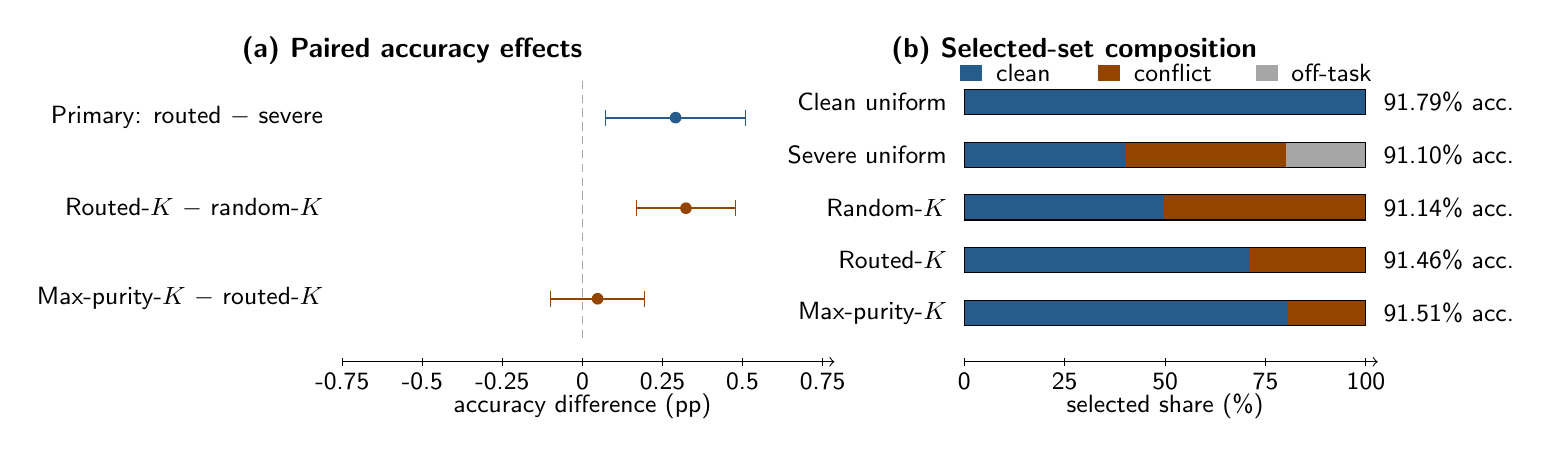
\begin{tikzpicture}[font=\sffamily\fontsize{9}{10}\selectfont]
\node[anchor=west,font=\sffamily\bfseries] at (0,4.7) {(a) Paired accuracy effects};
\draw[->] (1.400,0.75) -- (7.650,0.75);
\node at (4.450,0.18) {accuracy difference (pp)};
\draw[densely dashed,kafagray] (4.450,1.05) -- (4.450,4.35);
\draw (1.400,0.70)--(1.400,0.80) node[below=2pt] {-0.75};
\draw (2.417,0.70)--(2.417,0.80) node[below=2pt] {-0.5};
\draw (3.433,0.70)--(3.433,0.80) node[below=2pt] {-0.25};
\draw (4.450,0.70)--(4.450,0.80) node[below=2pt] {0};
\draw (5.467,0.70)--(5.467,0.80) node[below=2pt] {0.25};
\draw (6.483,0.70)--(6.483,0.80) node[below=2pt] {0.5};
\draw (7.500,0.70)--(7.500,0.80) node[below=2pt] {0.75};
\node[anchor=east] at (1.280,3.850) {Primary: routed $-$ severe};
\draw[line width=0.8pt,kafablue] (4.741,3.850)--(6.524,3.850);
\draw[kafablue] (4.741,3.750)--(4.741,3.950) (6.524,3.750)--(6.524,3.950);
\fill[kafablue] (5.633,3.850) circle (2.1pt);
\node[anchor=east] at (1.280,2.700) {Routed-$K$ $-$ random-$K$};
\draw[line width=0.8pt,kafaorange] (5.140,2.700)--(6.388,2.700);
\draw[kafaorange] (5.140,2.600)--(5.140,2.800) (6.388,2.600)--(6.388,2.800);
\fill[kafaorange] (5.764,2.700) circle (2.1pt);
\node[anchor=east] at (1.280,1.550) {Max-purity-$K$ $-$ routed-$K$};
\draw[line width=0.8pt,kafaorange] (4.043,1.550)--(5.241,1.550);
\draw[kafaorange] (4.043,1.450)--(4.043,1.650) (5.241,1.450)--(5.241,1.650);
\fill[kafaorange] (4.642,1.550) circle (2.1pt);
\node[anchor=west,font=\sffamily\bfseries] at (8.25,4.7) {(b) Selected-set composition};
\draw[->] (9.300,0.75)--(14.550,0.75);
\node at (11.850,0.18) {selected share (\%)};
\fill[kafablue] (9.25,4.32) rectangle +(0.28,0.20); \node[anchor=west] at (9.58,4.42) {clean};
\fill[kafaorange] (11.0,4.32) rectangle +(0.28,0.20); \node[anchor=west] at (11.33,4.42) {conflict};
\fill[kafagray] (13.0,4.32) rectangle +(0.28,0.20); \node[anchor=west] at (13.33,4.42) {off-task};
\draw (9.300,0.70)--(9.300,0.80) node[below=2pt] {0};
\draw (10.575,0.70)--(10.575,0.80) node[below=2pt] {25};
\draw (11.850,0.70)--(11.850,0.80) node[below=2pt] {50};
\draw (13.125,0.70)--(13.125,0.80) node[below=2pt] {75};
\draw (14.400,0.70)--(14.400,0.80) node[below=2pt] {100};
\node[anchor=east] at (9.200,4.050) {Clean uniform};
\fill[kafablue] (9.300,3.890) rectangle (14.400,4.210);
\fill[kafaorange] (14.400,3.890) rectangle (14.400,4.210);
\fill[kafagray] (14.400,3.890) rectangle (14.400,4.210);
\draw (9.300,3.890) rectangle (14.400,4.210);
\node[anchor=west] at (14.500,4.050) {91.79\% acc.};
\node[anchor=east] at (9.200,3.380) {Severe uniform};
\fill[kafablue] (9.300,3.220) rectangle (11.352,3.540);
\fill[kafaorange] (11.352,3.220) rectangle (13.384,3.540);
\fill[kafagray] (13.384,3.220) rectangle (14.400,3.540);
\draw (9.300,3.220) rectangle (14.400,3.540);
\node[anchor=west] at (14.500,3.380) {91.10\% acc.};
\node[anchor=east] at (9.200,2.710) {Random-$K$};
\fill[kafablue] (9.300,2.550) rectangle (11.833,2.870);
\fill[kafaorange] (11.833,2.550) rectangle (14.400,2.870);
\fill[kafagray] (14.400,2.550) rectangle (14.400,2.870);
\draw (9.300,2.550) rectangle (14.400,2.870);
\node[anchor=west] at (14.500,2.710) {91.14\% acc.};
\node[anchor=east] at (9.200,2.040) {Routed-$K$};
\fill[kafablue] (9.300,1.880) rectangle (12.922,2.200);
\fill[kafaorange] (12.922,1.880) rectangle (14.400,2.200);
\fill[kafagray] (14.400,1.880) rectangle (14.400,2.200);
\draw (9.300,1.880) rectangle (14.400,2.200);
\node[anchor=west] at (14.500,2.040) {91.46\% acc.};
\node[anchor=east] at (9.200,1.370) {Max-purity-$K$};
\fill[kafablue] (9.300,1.210) rectangle (13.404,1.530);
\fill[kafaorange] (13.404,1.210) rectangle (14.400,1.530);
\fill[kafagray] (14.400,1.210) rectangle (14.400,1.530);
\draw (9.300,1.210) rectangle (14.400,1.530);
\node[anchor=west] at (14.500,1.370) {91.51\% acc.};
\end{tikzpicture}
\end{document}
